 \documentclass[t,14pt]{beamer}
 %
 % Packages pour le français
 \usepackage[T1]{fontenc} 
 \usepackage[utf8]{inputenc}
 \usepackage[frenchb]{babel}
 %
 % pour un pdf lisible à l'écran
 % il y a d'autres choix possibles 
 \usepackage{pslatex}
\usetheme{Singapore}
  \usecolortheme{rose}
  \setbeamertemplate{blocks}[rounded][shadow=true]

\title{\textbf{\textit{Extraction et Analyse d'Images}}}
\subtitle{PED}
\author{\scriptsize{Manson Tomy\\
		Mestreau Nicolas\\
		Ridel Fabien\\
		Wen Jun\\
		\vspace{10mm}
		Encadrant : \\
		Laviole Jérémy\\
		}}
\institute{\tiny Université de Bordeaux 1}



\begin{document}

\frame{\titlepage}

%% part 1 - Jun
\section[Presentation]{Presentation}
\AtBeginSection[]{
\begin{frame}{Table of contents}
\small \tableofcontents[currentsection, hideothersubsections]
\end{frame}
}

\begin{frame}{Presentation du projet}
\begin{center}
\vspace{5mm}
Le but de ce projet est la création d'une bibliothèque de vision par l'ordinateur et analyse d'image.

\end{center}
\begin{itemize}
\item Entrée: un flux vidéo de dessin et des images qualitées hautes.
\item Sorti: un image de dessin ou pictogramme .
\end{itemize}
\end{frame}

\begin{frame}{Objectifs}
\begin{center}
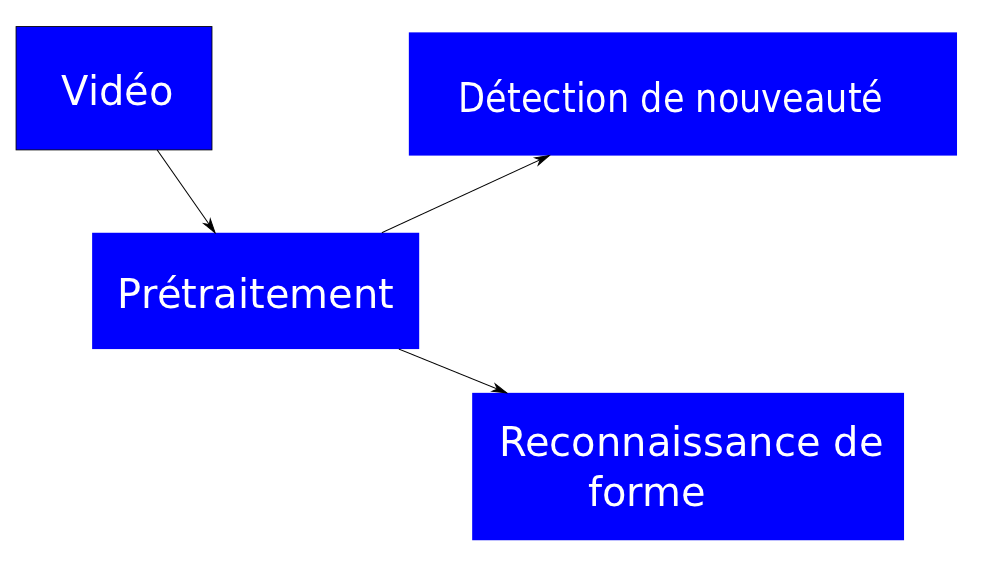
\includegraphics[scale=0.2]{images/dessin.png} 
\\ schéma de processus
\end{center}
\begin{itemize}
\item Augementer la qualité d'image la plus haute possible.
\item Récupérer les nouveautés du dessin.
\item Détecter les formes simples. 
\end{itemize}
\end{frame}


\begin{frame}{Application }
\vspace{2mm}
\begin{itemize}
\item Jeu vidéo Réalité Augementé

\begin{center}
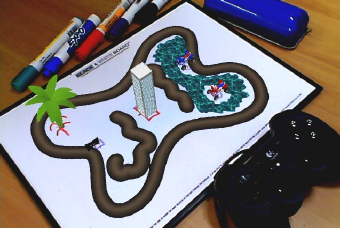
\includegraphics[scale=0.5]{images/sketchchasser.png}
\textit{\\sketchchasser}
\end{center}
\item Auto-scanner 
\end{itemize}
\end{frame}

%% part 2 - Fabien
\section[Pré-traitement]{Pretraitement}
\vspace{5mm}
\begin{frame}{Filtres}
\vspace{5mm}
\begin{itemize}[<+->]
\item Adaptation Tracker to Saliency descriptors (Saliency maps)
\item Integration tools in a unique software
\end{itemize}
\end{frame}

%% part 3 - Nicolas
\section[Détection de Pictogrammes]{Template Detector}
\begin{frame}{Objectif}
\vspace{5mm}
\begin{itemize}
\item Développer un logiciel qui détecte des pictogrammes dans un flux vidéo.
\item Utilisation de templates représentant les pictogrammes.
\vspace{5mm}
\begin{center}
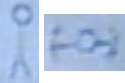
\includegraphics[scale=0.66]{images/templates.png}
\end{center}
\end{itemize}
\end{frame}

\begin{frame}{Méthode utilisée}
\vspace{5mm}
\begin{itemize}
\item Template Matching
\item Principe : 
\begin{center}
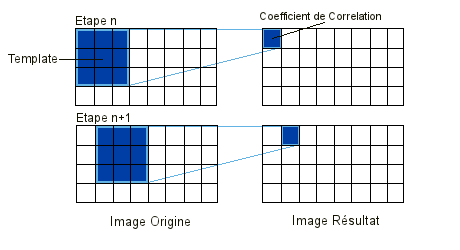
\includegraphics[scale=0.66]{images/templateMatching.png}
\end{center}
\end{itemize}
\end{frame}
			
\begin{frame}{Problème rencontré}
\vspace{5mm}
\begin{itemize}
\item \texttt{cvMatchTemplate} -> Carte de corrélation
\item Récupération du meilleur résultat
\item Difficulté pour déterminer un seuil d'acceptation
\end{itemize}
\end{frame}	

\begin{frame}{Résultats obtenus}
\vspace{5mm}
\begin{center}
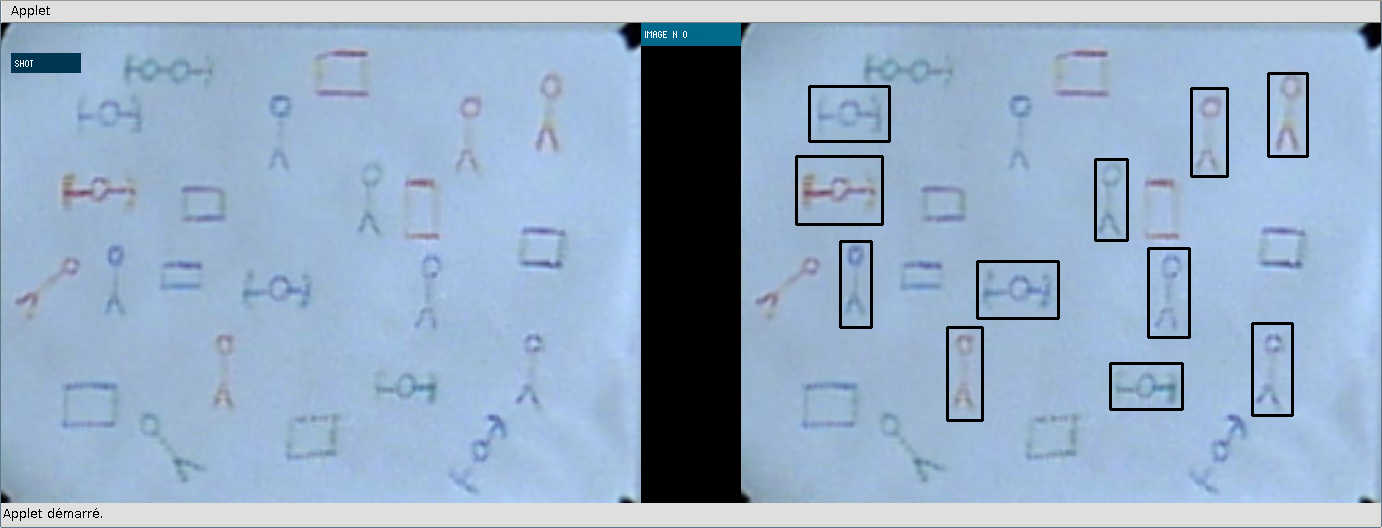
\includegraphics[width=\textwidth]{images/capture1.png}
\end{center}
\end{frame}

\begin{frame}{Résultats obtenus}
\vspace{5mm}
\begin{center}
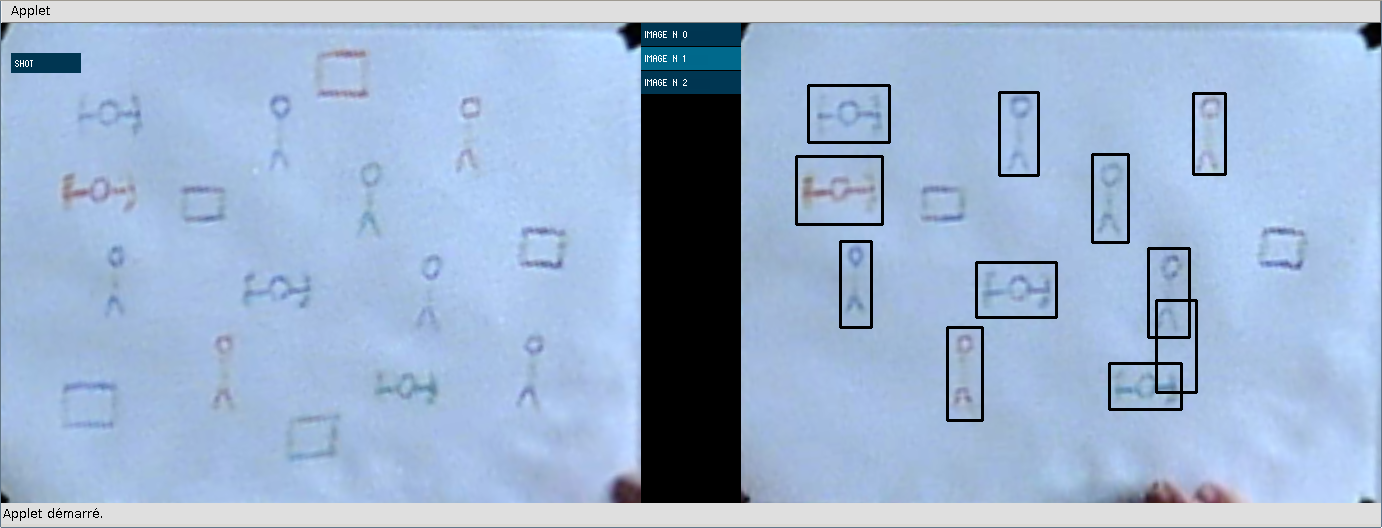
\includegraphics[width=\textwidth]{images/capture2.png}
\end{center}
\end{frame}

\begin{frame}{Méthode alternative}
\vspace{5mm}
\begin{itemize}
\item SURF
\item Intérêt : Non affecté par rotation et mise à l'échelle 
\item Problème : Qualité vidéo trop basse -> Trop peu de marqueurs détectés
\end{itemize}
\end{frame}
	
%% part 4 - Tomy
\section[Extraction de nouveautés]{Feature Extractor}
	\begin{frame}{Difficulties}
		\vspace*{5mm}
	\begin{itemize}
	\item Libraries installation
	\item Memory management
	\item Visualisation
	\end{itemize}
	\end{frame}
	
\section[Conclusion]{Conclusion}
	\begin{frame}{Conclusion}
		\vspace*{5mm}
		\begin{itemize}
		\item Software partially working
		\item A bad choice of buffer implementation
		\item Tests not done due to a lack of time
		\end{itemize}
	\end{frame}

\end{document}
